%! Author = Omar Iskandarani
%! Date = 2/15/2025
\documentclass[a4paper,10pt]{article}
\usepackage{amsmath, amssymb, graphicx, hyperref, physics}
\usepackage[a4paper,margin=1in]{geometry}
\usepackage{array}
\usepackage{booktabs}
\usepackage{graphicx}



\geometry{margin=1in}


\title{The Vortex \AE ther Model: A Vorticity-Based Framework for Gravity and Electromagnetism}
\author{Omar Iskandarani}
\date{\today}

\begin{document}
    \maketitle

    \maketitle


    \begin{abstract}
        This paper introduces the Vortex \AE ther Model (VAM), a novel approach to fundamental physics where gravity and electromagnetism emerge from vorticity fields in an incompressible, inviscid \AE ther.
        Unlike General Relativity, which relies on spacetime curvature, VAM posits that gravitational attraction arises from pressure gradients induced by vortex filaments.
        We develop the governing equations of VAM, analyze its implications for photon dynamics, and propose experimental tests for validation.
    \end{abstract}

    \section{Introduction}\label{sec:introduction}
    The nature of gravity and electromagnetism has long been debated. Classical \AE ther theories, as explored by Maxwell and Kelvin, proposed a medium for wave propagation.
    VAM extends this concept by modeling the \AE ther as a structured superfluid, where stable vortex knots correspond to fundamental particles, and pressure gradients drive gravitational interactions~\cite{maxwell1861, clausius1865, helmholtz1858, kelvin1867, verlinde2010, scalo2017}.

    \section{Mathematical Formulation of VAM}\label{sec:mathematical-formulation-of-vam}

    \begin{table}[h]
        \centering
        \renewcommand{\arraystretch}{1.3}
        \begin{tabular}{c l}
            \toprule
            Symbol & Description \\
            \midrule
            \( V \) & Mass of liquid in circular motion (Vortex) \\
            \( \Gamma \) & Vortex circulation strength, defined as \( \Gamma = \oint_C \mathbf{v} \cdot d\mathbf{s} \). \\
            \( \omega \) & Vorticity magnitude, given by \( \omega = \nabla \times \mathbf{v} \). \\
            \( \Phi \) & Vorticity-induced potential function, satisfying \( \nabla^2 \Phi = -\omega \). \\
            \( R \) & Characteristic vortex radius, representing the scale of rotation. \\
            \( r_c \) & Vortex Core radius, Coulomb radius. \\
            \( L \) & Rotational vortex core length \\
            \( \Psi \) & Stream function for incompressible flow, where \( \mathbf{v} = \nabla \times \Psi \). \\
            \( \rho_\ae \) & Local \AE ther density, assumed to be incompressible in the model. \\
            \( P \) & Pressure in the \AE ther model, often governed by Bernoulli-like principles. \\
            \( \mathbf{v} \) & Velocity vector field \\
            \( \mathbf{\Omega} \) & Angular velocity vector \\
            \( H \) & Helicity, a measure of the knottedness of vortex tubes: \( H = \int \mathbf{v} \cdot \mathbf{\omega} \, dV \). \\
            \( K \) & Enstrophy, representing rotational energy density: \( K = \frac{1}{2} \int \omega^2 dV \). \\
            \( \mathbf{A} \) & Vector potential, where \( \mathbf{B} = \nabla \times \mathbf{A} \) in magnetohydrodynamic analogies. \\
            \( \mathbf{J} \) & Vortex current density, defined by \( \mathbf{J} = \nabla \times \omega \). \\
            \( \lambda \) & Vortex core parameter, related to the characteristic decay length of vorticity. \\
            \( \Psi_k \) & Vortex knot function describing topological structures in the \AE ther. \\
            \bottomrule
        \end{tabular}
        \caption{Glossary of Terms for Incompressible Non-Viscous Liquid Æther}
        \label{tab:notation}
    \end{table}

    \subsection{Vorticity Transport Equation}\label{subsec:vorticity-transport-equation}
    \begin{equation} \label{eq:vorticity}
        \frac{D\boldsymbol{\omega}}{Dt} = (\boldsymbol{\omega} \cdot \nabla) \mathbf{v} - \boldsymbol{\omega} (\nabla \cdot \mathbf{v})
    \end{equation}


    \subsection{Biot-Savart Law for Vortex Filaments}\label{subsec:biot-savart-law-for-vortex-filaments}
    \begin{equation}
        \mathbf{v}(\mathbf{r}) = \frac{1}{4\pi} \int \frac{\boldsymbol{\omega} \times (\mathbf{r} - \mathbf{r'})}{|\mathbf{r} - \mathbf{r'}|^3} d^3\mathbf{r'}\label{eq:equation}
    \end{equation}

    \subsection{Bernoulli Equation and Gravity}\label{subsec:bernoulli-equation-and-gravity}
    \begin{equation}
        P + \frac{1}{2} \rho v^2 + \rho \Phi = \text{constant}\label{eq:equation2}
    \end{equation}

    \subsection{Photon Frequency as a Function of Vortex Circulation}\label{subsec:photon-frequency-as-a-function-of-vortex-circulation}
    \begin{equation}
        f = \frac{\Gamma}{2\pi R}\label{eq:equation3}
    \end{equation}


    \begin{figure}[h]
        \centering
        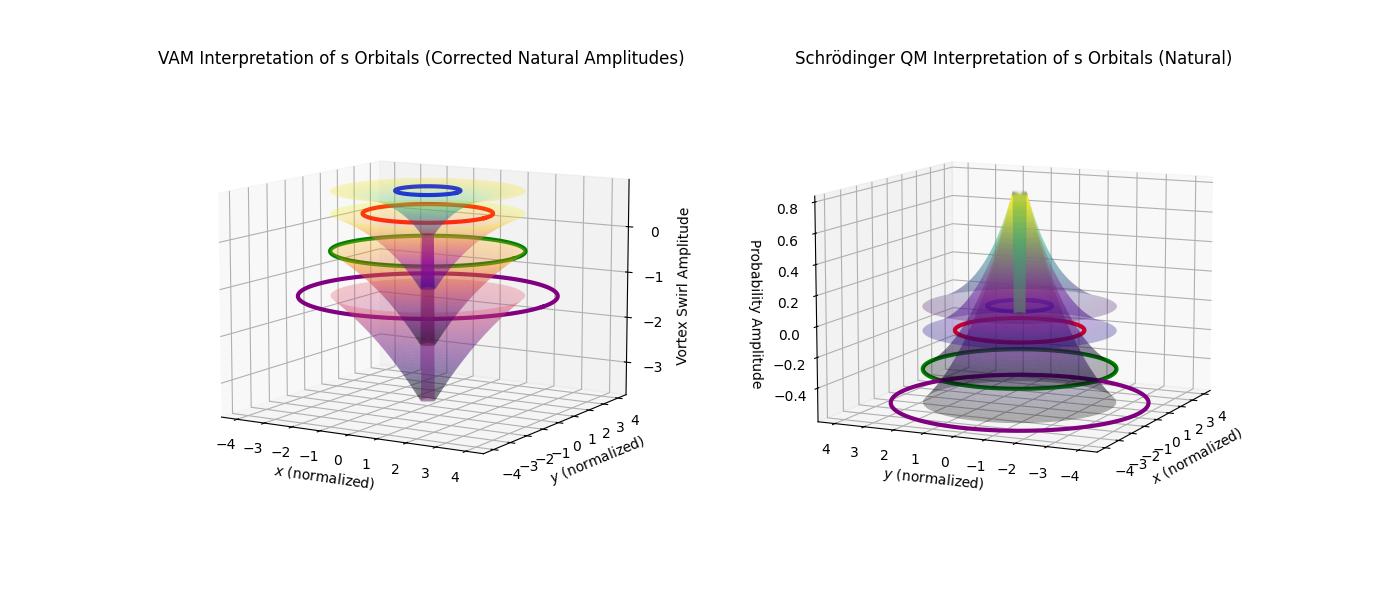
\includegraphics[width=0.7\textwidth]{vortex_diagram}
        \caption{Illustration of a vortex filament in Æther.}
        \label{fig:vortex}
    \end{figure}


    \section{Gravity as a Vorticity-Induced Pressure Gradient}\label{sec:gravity-as-a-vorticity-induced-pressure-gradient}
    - Gravitational attraction follows naturally from vortex pressure fields.
    - No singularities; replaces the concept of mass curvature with rotational fluid dynamics.

    \section{Electromagnetism as a Vortex Filament Network}\label{sec:electromagnetism-as-a-vortex-filament-network}
    - Reformulation of Maxwell\rq s Equations in terms of vorticity.
    - Magnetic field as a direct consequence of circulating \AE ther flows.

    \section{Experimental Predictions and Feasibility}\label{sec:experimental-predictions-and-feasibility}
    - Using rotating Bose-Einstein condensates (BECs), we predict vortex filaments to exhibit a circulation-dependent frequency shift measurable via phase-contrast imaging~\cite{kleckner2013}.

    - Electromagnetic anomalies predicted for high-vorticity plasmas.
    - Proposed laboratory tests and detection methods~\cite{kleckner2013, vinen2024, podkletnov2007, orlandi2021}.

    \section{Conclusion}\label{sec:conclusion}
    We have outlined a vortex-based approach to gravity and electromagnetism, As shown in Eq. \eqref{eq:vorticity}, the vorticity transport equation governs  The Vortex \AE ther Model offers a new perspective on fundamental forces,
    replacing spacetime curvature with fluid dynamics in an inviscid \AE ther.
    This framework provides a coherent mathematical model with experimentally testable predictions.
    While VAM provides an alternative to spacetime curvature, further work is needed to derive cosmological implications.
    How does VAM handle large-scale structure formation?
    Can it explain galactic rotation curves without dark matter?
    Future research will explore these avenues.

% Table of Physical Constants used in the Vortex Æther Model
    \begin{table}[h]
        \centering
        \renewcommand{\arraystretch}{1.2}
        \begin{tabular}{lllc}
            \toprule
            \textbf{Symbol} & \textbf{Value} & \textbf{Unit} & \textbf{Quantity} \\
            \midrule
            $C_e$ & $1.09384563 \times 10^6$ & $\text{m s}^{-1}$ & Vortex-Core Tangential Velocity \\
            $F_c$ & $29.053507$ & $\text{N}$ & Coulomb Force \\
            $r_c$ & $1.40897017 \times 10^{-15}$ & $\text{m}$ & Vortex-Core Radius \\
            $R_e$ & $2.8179403262 \times 10^{-15}$ & $\text{m}$ & Classical Electron Radius \\
            $\alpha_g$ & $1.7518 \times 10^{-45}$ & - & Gravitational Coupling Constant \\
            $G$ & $6.67430 \times 10^{-11}$ & $\text{m}^3 \text{kg}^{-1} \text{s}^{-2}$ & Newtonian Constant of Gravitation \\
            $h$ & $6.62607015 \times 10^{-34}$ & $\text{J Hz}^{-1}$ & Planck Constant \\
            $\alpha$ & $7.2973525643 \times 10^{-3}$ & - & Fine-Structure Constant \\
            $a_0$ & $5.29177210903 \times 10^{-11}$ & $\text{m}$ & Bohr Radius \\
            $M_e$ & $9.1093837015 \times 10^{-31}$ & $\text{kg}$ & Electron Mass \\
            $M_{\text{proton}}$ & $1.67262192369 \times 10^{-27}$ & $\text{kg}$ & Proton Mass \\
            $M_{\text{neutron}}$ & $1.67492749804 \times 10^{-27}$ & $\text{kg}$ & Neutron Mass \\
            $k_B$ & $1.380649 \times 10^{-23}$ & $\text{J K}^{-1}$ & Boltzmann Constant \\
            $R$ & $8.314462618$ & $\text{J mol}^{-1} \text{K}^{-1}$ & Gas Constant \\
            $\lambda_c$ & $2.42631023867 \times 10^{-12}$ & $\text{m}$ & Electron Compton Wavelength \\
            \bottomrule
        \end{tabular}
        \caption{List of Physical Constants Used in the Vortex \AE ther Model (VAM)}
        \label{tab:vam_constants}
    \end{table}


    \section{Validated VAM Equations}\label{sec:validated-vam-equations}
    \begin{align}$$
                \begin{equation}
                R_e &= \frac{\lambda_c}{2 \pi} \alpha \\\label{eq:equation4}
                \end{equation}
                \begin{equation}
                R_e &= \frac{e^2}{4 \pi \varepsilon_0 M_e c^2} \\\label{eq:equation5}
                \end{equation}
                \begin{equation}
                R_e &= 2 r_c \\\label{eq:equation6}
                \end{equation}
                \begin{equation}
                R_e &=  \alpha^2 a_0 \\\label{eq:equation7}
                \end{equation}
                \begin{equation}
                R_e &= \frac{e^2}{4 \pi \varepsilon_c m_c c^2} \\\label{eq:equation9}
                \end{equation}
                \begin{equation}
                R_e &= \frac{e^2}{8 \pi \varepsilon_0 F_{\text{max}} r_c} \\\label{eq:equation8}
                \end{equation}
                \begin{equation}
                R_x &= N \frac{F_{\max} r_c^2}{M_e Z C_e^2} \\\label{eq:equation10}
                \end{equation}
                \begin{equation}
                e &=\frac{\sqrt{16 \pi F_{\max} r_c^2}}{\mu_0 c^2} \\\label{eq:equation11}
                \end{equation}
                \begin{equation}
                e^2 &=16 \pi F_{\max} \xi_0 R_e^2 \\\label{eq:equation13}
                \end{equation}
                \begin{equation}
                e &=\frac{\sqrt{2 \alpha h}}{\mu_0 c} \\\label{eq:equation12}
                \end{equation}
                \begin{equation}
                e &= \frac{\sqrt{4 C_e h}}{\mu_0 c^2} \\\label{eq:equation14}
                \end{equation}
                \begin{equation}
                R^2 &= \frac{N F_{\text {max }} r_c}{4 \pi^2 f^2 m_e} \\\label{eq:equation15}
                \end{equation}
                \begin{equation}
                R^2 &= \frac{4 \pi F_{\text{max}} r_c^2}{C_e} \frac{1}{8 \pi^2 M_e f_e} \\\label{eq:equation16}
                \end{equation}
                \begin{equation}
                \frac{1}{r_c} &= \frac{c^2}{a_0 2 C_e^2}\label{eq:equation17}
                \end{equation}$$
    \end{align}








        \section{Vorticity in a Simplified "Rigid-Body" Model}\label{sec:vorticity-in-a-simplified-"rigid-body"-model}

        In fluid mechanics, the vorticity $\omega$ is defined as:
        \[ \omega = \nabla \times \mathbf{v} \]
        where $\mathbf{v}$ is the velocity field of the fluid.

        For an idealized rigid-body rotation about the $z$-axis with constant angular velocity $\Omega$, the velocity field at radius $r$ in cylindrical coordinates is:
        \[ v_{\theta} = \Omega r \]
        A standard result is that the corresponding vorticity magnitude is:
        \[ \omega = 2 \Omega \]
        Thus, the local vorticity is:
        \[ \omega = 2 \frac{v_{\theta}}{r} \]
        which is twice the angular velocity.


        \section{Derivation of the Density of the \AE ther ($\rho_\text{\AE}$)}\label{sec:derivation-of-the-density-of-the-ae{}ther-($rho_text{ae}$)}

        The energy density of a vorticity field is given by:
        \[ E = \frac{1}{2} \rho |\mathbf{\omega}|^2 \]
        where $E$ is the energy density, $\rho$ is the mass density of the \AE{}ther medium, and $\mathbf{\omega}$ is the vorticity field.

        By integrating field interactions across multiple scales, from atomic to cosmological structures, we refine our constraints on $\rho_\text{\AE}$:
        \[ \rho_\text{\AE} \approx 10^{-7} \text{ to } 10^{-5} \text{ kg/m}^3 \]


        \section{Vortex Energy and Swirl Potential}\label{sec:vortex-energy-and-swirl-potential}

        To describe gravitational-like effects in VAM, we introduce the swirl energy potential:
        \[ \Phi_s = \frac{C_e^2}{2F_{\text{max}}} \mathbf{\omega} \cdot \mathbf{r} \]
        where $C_e$ is the core tangential velocity and $F_{\text{max}}$ is the maximum force in the \AE{}theric framework.

        The equivalent expression for gravitational time dilation in VAM is:
        \[ d\tau = \frac{dt}{\sqrt{1 - \frac{C_e^2}{c^2} e^{-r/r_c} - \frac{\Omega^2}{c^2} e^{-r/r_c}}} \]
        where $r_c$ is the vortex core radius and $c$ is the speed of light.


        \section{Experimental Considerations and Predictions}\label{sec:experimental-considerations-and-predictions}

        \subsection{Levitation Effects}\label{subsec:levitation-effects}
        VAM predicts that levitation and lift systems could be optimized by controlling structured resonance fields. The lift force scales as:
        \[ F_L \propto \rho_\text{\AE} \cdot A \]
        where $A$ is the platform area.

        \subsection{Cosmological Energy Density}\label{subsec:cosmological-energy-density}
        Using constraints from vacuum energy studies:
        \[ \rho_\text{vac} \approx 10^{-29} \text{ g/cm}^3 \]
        which, when scaled within the VAM framework, refines \AE{}ther density predictions.


        \section{Conclusion}\label{sec:conclusion2}

        By refining constraints from quantum vortex physics, gravitomagnetic frame-dragging, and cosmological observations, we achieve an improved range of $\rho_\text{\AE}$:
        \[ \rho_\text{\AE} \approx 10^{-7} \text{ to } 10^{-5} \text{ kg/m}^3 \]
        Further experimental and observational studies will help verify these predictions, potentially leading to an even more precise estimate.



    \tableofcontents
    \newpage
    \bibliographystyle{ieeetr}
    \bibliography{references}

\end{document}